\chapter{Results}

\section{Model Diagnostics}
120,000 (15,000 burn-in) samples of posterior distribution were obtained using the adaptive Markov Chain Monte Carlo algorithm described in Chapter 3. Figure \ref{diagnostics} shows trace and autocorrelation plots for a randomly selected marginal posteriors of $\beta$ and $\phi$, as well as the marginal posteriors for both $s$ and $\tau$. 

\begin{figure}
\centering
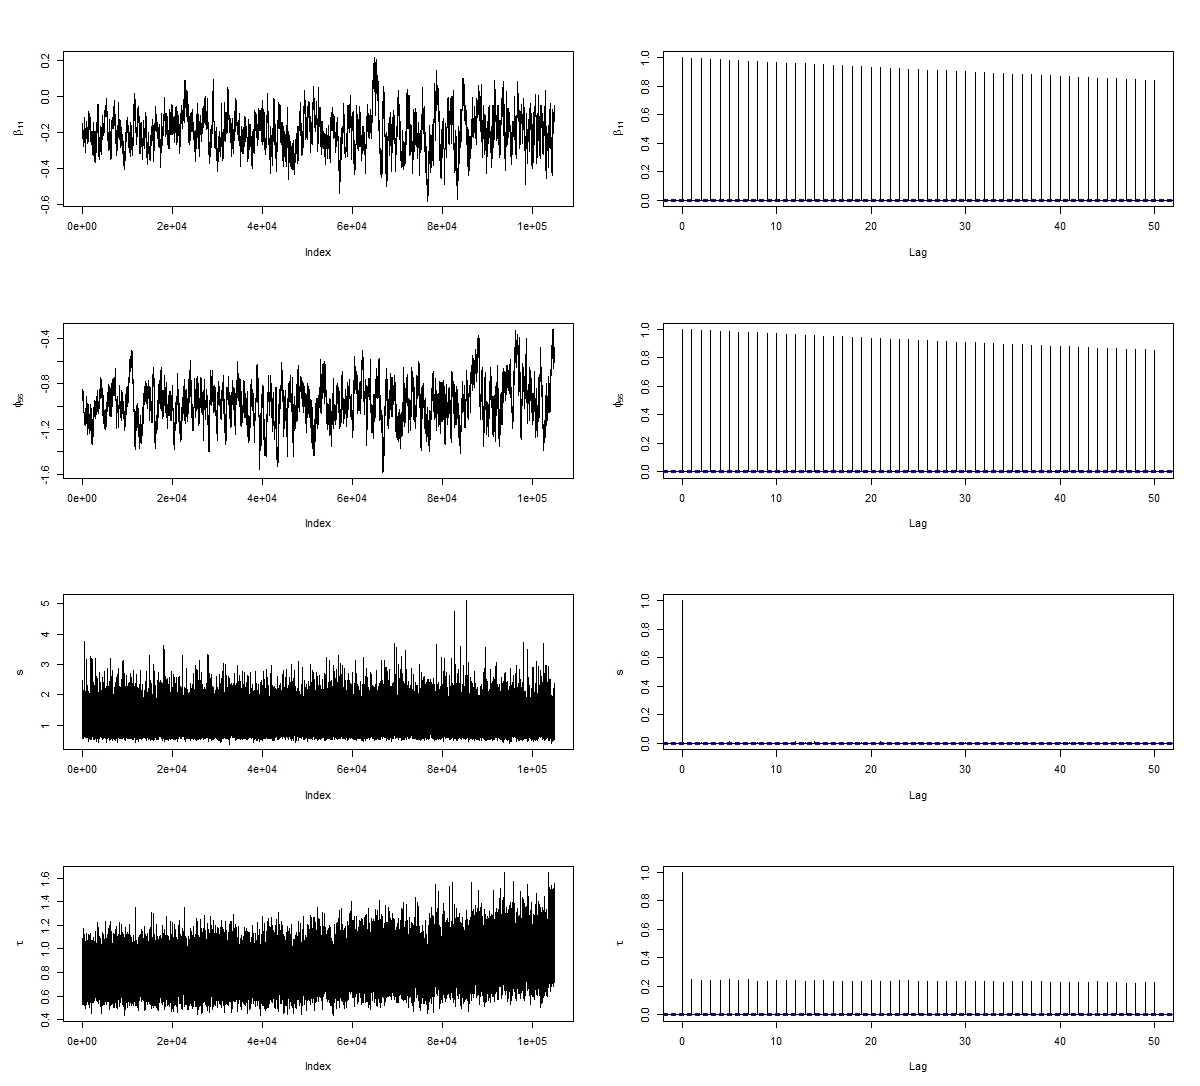
\includegraphics[width=.70\textwidth]{diagnostics.jpeg}
\caption{Trace and autocorrelation plots to assess convergence}
\label{diagnostics}
\end{figure}

Marginal distributions for nearly all $\beta$'s and $\phi$'s have very high autorrelation that can be seen in Figure \ref{diagnostics}. Despite the high autocorellation for the $\beta$'s and the $\phi$'s, the trace plots show that the MCMC has sufficiently explored the space of our parameters. The trace and autocorrelation plots for $s$ and $\tau$ indicate more than adquate convergence. We verify convergence of the MCMC using Monte Carlo standard errors \citep{jones06}. All of the MCMC standard errors for the $\beta$'s were less than .01. All of the MCMC standard errors except three for $\phi$ were smaller than .01. \\

To verify that the fitted model fits the data well, posterior predictive checks were used. Figure \ref{predictive} shows 95\% predictive intervals for each of the 207 road segments on the I35. Of the 207 intervals, 197 contain the observed value ($\approx 95\%$ coverage).

\begin{figure}[h]
\centering
\includegraphics[width=.70\textwidth]{predictivei35.pdf}
\caption{Posterior predictive intervals: blue dots indicate the observed number of crashes fell within a 95\% interval, while red dots indicate the observed crashes did not fall within the interval.}
\label{predictive}
\end{figure}



\section{Results:}
We are interested in what factors in the road lead to higher crash rates. As described in chapter 3, the $\beta$ coefficients give the relative risks of each road characteristic. If $\beta_p > 0$ then  increases in $x_p$ are associate with increased relative risk of accidents. \citet{betas} shows the central 95\% credible intervals for the intercept and each of the 11 covariates. Four covariates are above zero: (1) poor pavement conditions, (2) small and/or variable median width, (3) road width, and (4) right shoulder width. Small median width in particular stands out as having a large, positive association with increased risk of accidents. Small median widths are typically associated with highways in highly populated areas that have high volumes of traffic. Equation \eqref{Es} alone was unable to capture the effect of increased traffic.



\begin{table}[!htbp] \centering 
  \caption{} 
  \label{beta} 
\begin{tabular}{@{\extracolsep{5pt}} lcc} 
\\[-1.8ex]\hline 
\hline \\[-1.8ex] 
 & 2.5\% & 97.5\% \\ 
\hline \\[-1.8ex] 
(Intercept) & $$-$0.979$ & $$-$0.232$ \\ 
Adverse Pavement & $0.027$ & $0.064$ \\ 
Night Crashes & $$-$0.081$ & $$-$0.026$ \\ 
Median Width < 30 ft & $0.660$ & $1.075$ \\ 
Median Width Varies & $0.305$ & $0.557$ \\ 
No Median Barrier & $$-$0.218$ & $0.220$ \\ 
Left Shoulder Width & $$-$0.149$ & $$-$0.047$ \\ 
Left Shoulder Type `Other' & $$-$0.225$ & $$-$0.017$ \\ 
Surface Width (ft) & $$-$0.001$ & $0.047$ \\ 
Right Shoulder Width (ft) & $0.023$ & $0.134$ \\ 
Number of Lanes & $$-$0.382$ & $0.006$ \\ 
Lande Width (ft) & $$-$0.006$ & $0.010$ \\ 
\hline \\[-1.8ex] 
\end{tabular} 
\end{table} 

The covariates in the model did not capture all of the risk factors. For this reason it is important to include the spatial effects into the model. Figure \ref{spatial} includes estimated spatial effects for each road segment. We are most interested in areas where the spatial effects have a strong positive effect. 

\begin{figure}[h]
\centering
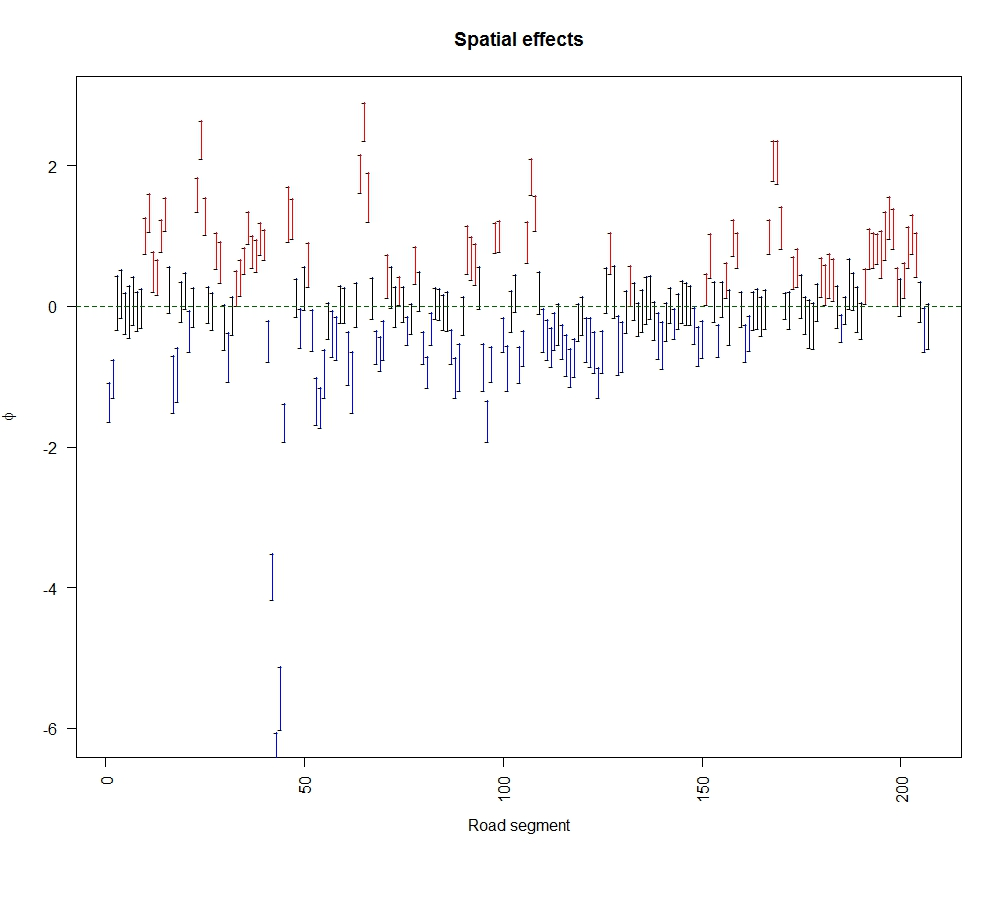
\includegraphics[width=.70\textwidth]{spatial.jpeg}
\caption{95\% credible intervals for the spatial effects. Blue lines indicate the intervals fall below zero while red lines indicate intervals are above zero. }
\label{spatial}
\end{figure}

Notice that segments 180-200 contain a high proportion of red segments. This indicates that these road segments have a higher relative crash rate than we would expect given the covariates. Segments 180-200 are associated with freeway segments in the Duluth-Superior metropolitan area. Reasons why crash rates are higher in Duluth than they should be could be for a variety of reasons including characteristics of the road such as high road curvature and steep roads or reasons could be socio-economic like a higher than normal drinking rate. 

Calculating $\mu_s=exp\{X_s'\beta + \phi_s\}$ gives us the relative risk (relative to the expected number of crashes $E_s$ from \eqref{Es}) for each road segment. Segments 24, 64,  65,  66, 107, 168, 169 (indicated in red in Figure \ref{relrisk} all have relative risk of over 2. These road segments should be examined to see why they have such a high risk. \\

\begin{figure}[!htbp] 
\centering
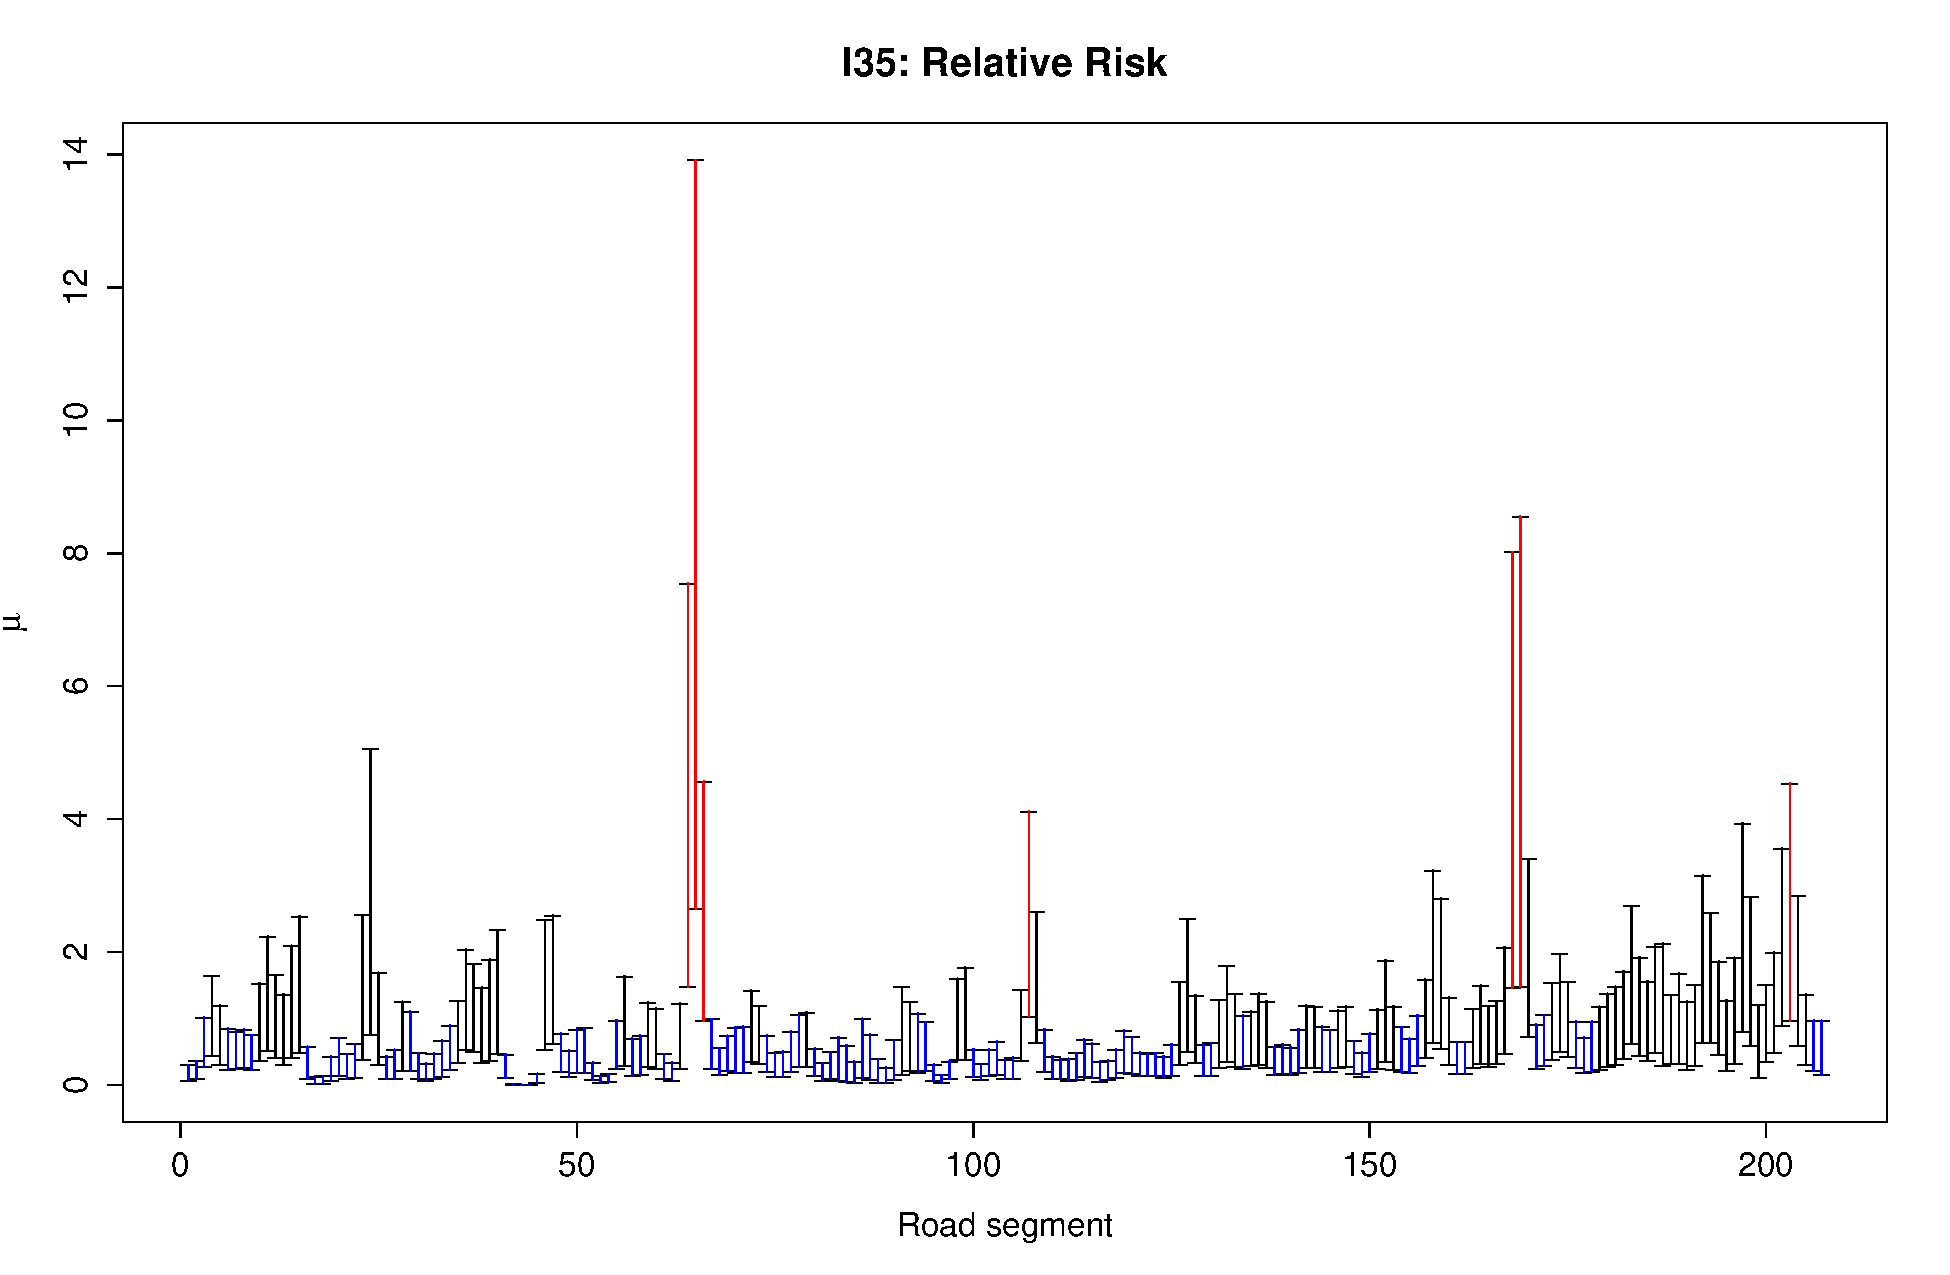
\includegraphics[width=.70\textwidth]{relrisk.pdf}
\caption{95\% credible intervals for the relative risks. Red lines indicate the estimated number of crashes is twice what it should be. }
\label{relrisk}
\end{figure}

